%!TEX root = ../draft.tex

\section{Discussion}
\label{sec:Discussion}
In this section, we discuss weaknesses of triangle closing mechanisms,
the effect of out-degree on network diameter and limitations \& potential
modifications of our model \texttt{ARW}.

\subsection{Dissecting the Triangle Closing Mechanism}
\label{ss:tc}

A set of network models (e.g., \texttt{SAN} \cite{gong2012evolution} \& \texttt{HK} \cite{holme2002growing})
use triangle closing mechanisms to generate networks with
varying average local clustering. However, our experimental results
in~\Cref{sub:Experimental Results} show that models that rely on triangle closing
cannot model local clustering distribution or bivariate degree-clustering
relationship accurately. To understand why, we examine the degree-clustering
relationship in the \texttt{APS} network, in~\Cref{fig:triangle_closing}.
\begin{figure}[h]
    \centering
    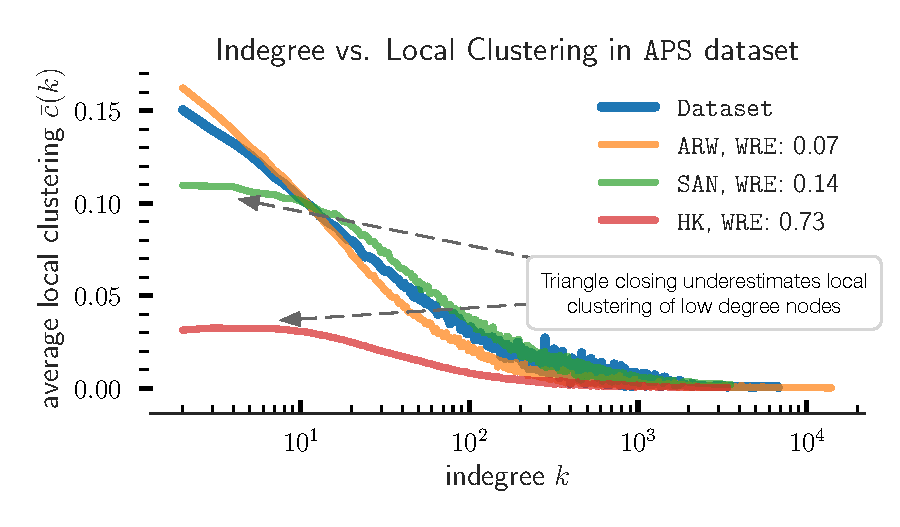
\includegraphics[width=.8\columnwidth]{triangle_closing}
    \caption{Triangle closing mechanisms used in \texttt{SAN} \texttt{HK} fail to
    model average local clustering of low in-degree nodes. In contrast,
    to accurately preserve local clustering, \texttt{ARW} uses {random walks} to visit
    low in-degree nodes and close triangles in their neighborhoods .}
    \label{fig:triangle_closing}
\end{figure}

\Cref{fig:triangle_closing} reveals that models based on triangle closing mechanisms,
\texttt{SAN} and \texttt{HK}, considerably underestimate the local clustering of
nodes that have low in-degree. This is because incoming nodes in \texttt{SAN} and \texttt{HK}
tend to close triangles in the neighborhood of high in-degree nodes to which they
connect via preferential attachment. Local clustering plateaus as in-degree decreases because
triangle closing along with preferential attachment fail to form connections in neighborhoods
of low in-degree nodes. In contrast, \texttt{ARW} accurately models the degree-clustering relationship
because incoming nodes initiate random walks and close triangles in neighborhoods of low in-degree
seed nodes chosen via \textsc{Select-Seed}.

\subsection{Effect of Out-degree on Network Diameter}
Extensive analyses \cite{hu2009evolution,mcglohon2011statistical,leskovec2005graphs} on evolving
real-world networks reveal two key temporal properties: network densification and diameter
shrinkage over time. Growth models can be adjusted to densify networks over time
by allowing node out-degree to increase super-linearly as a
function of network size. However, we lack a concrete understanding of existing
edge formation mechanisms' inability to preserve diameter shrinkage. Through our
analysis, we observe that the out-degree sequence of incoming nodes in
network models has a significant impact on effective diameter over time.
\begin{figure}[H]
 \vspace{-10pt}
 \centering
 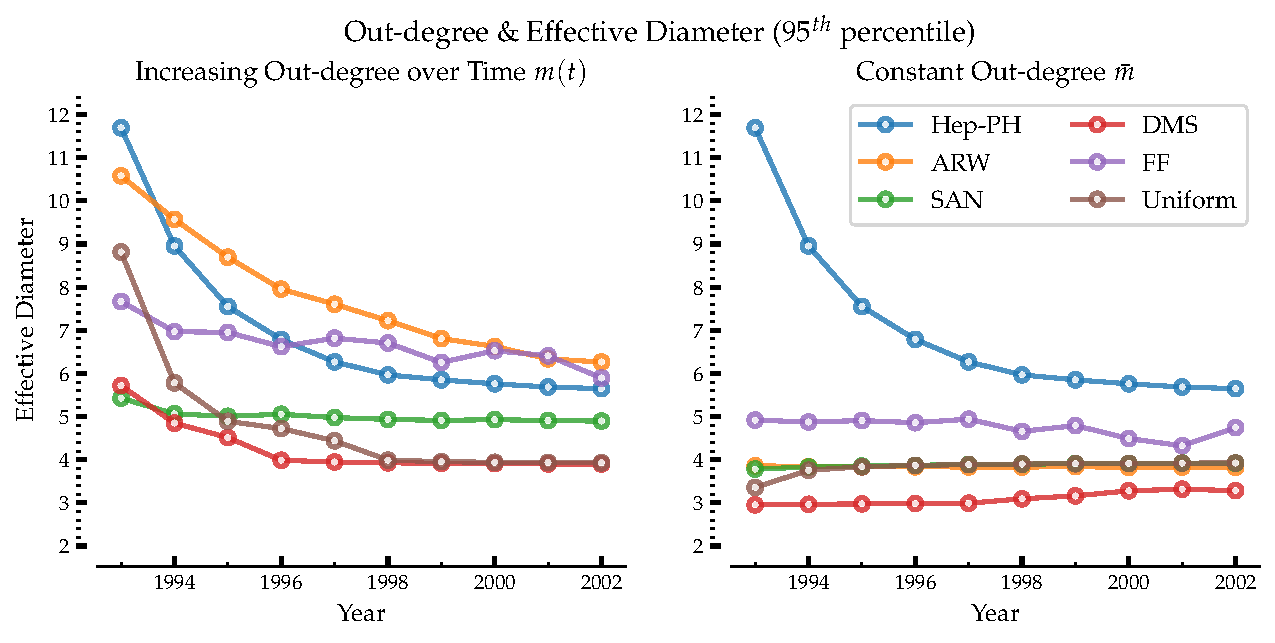
\includegraphics[width=\columnwidth]{outdegree_diameter}
 \caption{
 Effect of out-degree on effective diameter.
 The left subplot shows that increasing out-degree over time leads to diameter
 shrinkage for all models. The right subplot shows that
 constant out-degree sequence does not account for diameter
 shrinkage and consistently underestimates effective diameter of the \texttt{Hep-PH}
 network.}
 \label{fig:diameter}
 \vspace{-10pt}
\end{figure}

\Cref{fig:diameter} illustrates the effective diameter of network models fitted
to \texttt{Hep-PH} as a function of node out-degree sequence and time.
by increasing the
out-degree $m(t)$ of incoming nodes over time using the method described
in~\cref{sub:Model Fitting}, network models representative of key edge formation
mechanisms---\texttt{ARW}, \texttt{FF}, \texttt{DMS} \&
\texttt{SAN}---generate networks that exhibit diameter shrinkage. In particular,
\texttt{FF} \footnote{\texttt{FF} inherently increases out-degree over time
because incoming nodes ``burn'' through the network for duration in proportion
to the network size.} and \texttt{ARW} mirror the observed rate at which the
effective diameter shrinks over time.
When the out-degree $\bar{m}=n^{-1}\sum_i m(i)$ of incoming nodes is constant,
fitted networks, including Forest Fire (\texttt{FF}), cannot preserve
shrinking diameter; the effective diameter of the fitted models remain
consistently lower than that of \texttt{Hep-PH}.

Increasing out-degree over time can effectively incorporate diameter shrinkage
in all representative network models. This phenomena is best understood through
the simple \texttt{Uniform} null model, in which incoming nodes form edges to
existing nodes chosen uniformly at random. In the \texttt{Uniform} model, nodes with higher out-degree
have a greater probability of linking to existing
nodes that are structurally distant from each other. Consequently, over time,
incoming nodes with higher out-degree are more likely to bridge distant regions
of the network, reduce path length between existing nodes and subsequently
shrink effective diameter.

To summarize, our analysis indicates how increasing out-degree over time enables
existing models that rely on different edge formation processes to account for
diameter shrinkage.
% , an important temporal property of evolving real-world networks.

% \subsection{Connections to Vertex Copying}

\subsection{\texttt{ARW} Limitations}
We discuss three limitations of \texttt{ARW}. First, we  consider only
bibliographic  network datasets, as nodes form all edges at the time of joining.
This allows us to analyze edge formation in the absence of confounding edge
processes such as edge deletion and edge creation between existing nodes. We
plan to extend \texttt{ARW} to handle social networks, where individuals can
form edges at any time. One potential way is to incorporate random walks that
pause and resume intermittently, thus allowing for older nodes to connect with
more recent arrivals.
% Similarly, meta-path based random walks could potentially model interactions between nodes of different types in heterogeneous information networks.
Second, the out-degree $m(t)$ of incoming nodes in \texttt{ARW} rely on the
observed out-degree sequence, which might be unavailable in
datasets without fine-grained temporal data. In this case, \texttt{ARW}
can be adapted to rely on the prescribed range of densification exponent $\alpha_{\tiny \mbox{DPL}}$~\cite{leskovec2005graphs}
in real-world networks.
Since $e(t)=m(t)n(t)$, the power law relationship $e(t) \propto n(t)^{\alpha_{\tiny \mbox{DPL}}}$ between
number of edges $e(t)$ and nodes $n(t)$ at time $t$ implies that out-degree $m(t)$ must be proportional
to $n(t)^{\alpha_{\tiny \mbox{DPL}}-1}$.
Third, \texttt{ARW} focuses on modeling networks in which nodes have a single attribute.
The difficulty in incorporating multiple attributes into the edge formation mechanism rests
on how we measure attribute similarity. If two nodes are similar only when all their
attribute values are identical, we can simply create a new categorical attribute that encodes all
multiple attribute combinations and then directly apply \texttt{ARW}.
Additional analysis is necessary to identify definitions of attribute similarity that best
describe how multiple attributes influence individuals' edge formation processes.

% if attribute similarity two nodes are similar in proportion
% to the number of shared attribute values, then we need more subtle analysis.

% does not account for mixing patterns of numerical nodal attributessuch as publication year and age; we plan to conduct additional analysis on mixing
% patterns of numerical attributes in real-world networks to extend \texttt{ARW} in
% this direction.

% First, \texttt{ARW} does not preserve the average
% path length distribution of real-world networks. This is because the random walk
% mechanism is inherently local and does not form {long-range connections} to bridge
% distant regions of the network. Preliminary experiments on forming ``structural bridges''
% by initiating multiple random walks for every node indicate a tradeoff
% between modeling small average path length and high local clustering.

% \section{Limitations}
% Now, we discuss the limitations of our work. First, our work is limited to
% bibliographic datasets because of availibility of temporal data. We use the
% temporal out-degree sequence of incoming nodes in the network to model the
% network growth. In absence of temporal information, our growth model can be
% adapted by relying on the densification power law exponent. Second, our random
% walk model is sensitive to the initial graph. Since random walks explore the
% locality of a network and cannot access the entire network , the initial graph
% should have a giant weakly connected component. We recognise that the
% intialization problem can be addressed by having non-local source of information
% such as multiple seed nodes. Third, we note that our model fails to preserve
% certain network properties such as path length distribution. This is because
% our model does not account for nodes that serve as ``local bridges'' in the network.
% Modeling local and global processes simulatenously in a joint random walk model
% should lead to preservation of the discussed key network properties.


% \subsection{Measurement of Global Network Properties}
% Despite their widespread usage, summary statistics of global
% network properties such as global assortativity and average clustering have limited representative
% power. Unlike point estimates, distributional properties reveal variance, skewness and anomalies
% in network data.
% Notably, understanding local processes via distributional network properties
% guided the development of \texttt{ARW}, which consists of entirely \textit{local} processes
% that do not rely on global information (e.g. fitness values of all nodes).
% For instance, the \textit{skewed} clustering distribution and the relationship between clustering and
% degree necessitated the jump parameter $p_j$ in our model. The structural constraints imposed by the jump
% parameter amplify the effect of triadic closure and preserve high clustering
% observed in neighborhoods of low degree nodes.
% % Similarly, the variance in the
% % local assortativity distribution of real-world networks necessitated additional
% % stochasticity in the edge formation mechanism. As shown in
% % \cref{subsec:LocalMixing}, \texttt{ARW} accurately models varying local mixing
% % patterns because we augment seed selection to pick similar/dissimilar nodes
% % probabilistically. As a result, incoming nodes with fixed preferences can
% % initiate random walks in neighborhoods with varying local content properties.
% To summarize, we believe that the analysis and evaluation of \textit{distributional}
% network properties is crucial to accurately model network structure.

